\documentclass[a4paper,12pt]{report}
\usepackage[utf8x]{inputenc}
\usepackage[brazil]{babel}
\usepackage[T1]{fontenc}
\usepackage{epstopdf}
%\DeclareGraphicsRule{.tif}{png}{.png}{`convert #1 `dirname #1`/`basename #1 .tif`.png}
\usepackage{tikz}
\hyphenation{li-vro tes-te cha-ve bi-blio-te-ca}
\hyphenation{co-men-t-rio re-fe-rn-cia}
\usetikzlibrary{positioning,shapes,shadows,arrows}

\linespread{1.5}
\pagestyle{plain}

% Title Page
\title{Trabalho de AD - Simulador}
\author{Bruno Lima Cardoso - 108055733 \\
  Daniel Santos Ferreira Alves - 107362161 \\
  Mariam dos Passos Afonso da Conceição - 104034913 \\
\\
\\
\\
\\
\\
Os integrantes do grupo participaram ativamente, de \\
forma remota ou presencial, de todas as etapas da elaboração \\
do trabalho: definição do funcionamento do simulador, \\
implementação do código, testes e produção do relatório.
\\
\\
\\
}

%DICAS
%expressões matemáticas sempre entre $
%underline x_{underline}
%expoente x^{expoente}
%expoente e underline x_{underline}^{expoente}

\begin{document}

%%%%%%%%%%%%%%%%%%%
% parte frontal
%%%%%%%%%%%%%%%%%%%

\maketitle

\begin{abstract}
\end{abstract}

\chapter*{Siglas}
\begin{list}{$\bullet$}{}
  \item[VA] - Variável Aleatória
  \item[]
\end{list}

\chapter*{Lista de Variáveis}
\begin{list}{$\bullet$}{}
  \item[$N_{q1}$] - Número de pessoas em espera na fila 1.
  \item[$N_{q2}$] - Número de pessoas em espera na fila 2.
  \item[$N_1$] - Número de pessoas na fila 1.
  \item[$N_2$] - Número de pessoas na fila 2.
  \item[$W_1$] - Tempo de espera da fila 1.
  \item[$W_2$] - Tempo de espera da fila 2.
  \item[$X_1$] - Tempo do primeiro serviço.
  \item[$X_2$] - Tempo do segundo serviço.
  \item[$T_1$] - Tempo total de execução da fila 1.
  \item[$T_2$] - Tempo total de execução da fila 2.
  \item[$\rho$] - Utilização.
\end{list}

\tableofcontents

\listoffigures

\listoftables

%%%%%%%%%%%%%
% Introdução
%%%%%%%%%%%%%
\chapter{Introdução}

\section{Funcionamento Geral do Simulador}
Testando texto.

Segunda linha.

\section{Eventos Escolhidos}

\section{Estruturas Internas Utilizadas}

\section{Geração das Variáveis Aleatórias (VA)}

\section{Linguagem}

\section{Escolha de Parâmetros}

\section{Especificação da Máquina}

\section{Informações Adicionais}

%%%%%%%%%%%%%
% Testes
%%%%%%%%%%%%%
\chapter{Testes de Correção}

%%%%%%%%%%%%%
% Fase transiente
%%%%%%%%%%%%%
\chapter{Estimação da Fase Transiente}

\section{Método de Estimação}

\section{Resultados do Processo}

%%%%%%%%%%%%%
% Análise
%%%%%%%%%%%%%
%tabelas com resultados e comentários pertinentes
\chapter{Análise e Desempenho}


%Mude o caminho e descomente
%``graphs/graph-2.png é o caminho relativo da figura a partir do .tex
%\begin{figure}[htbp]
%   \centering
%   \fbox{
%	   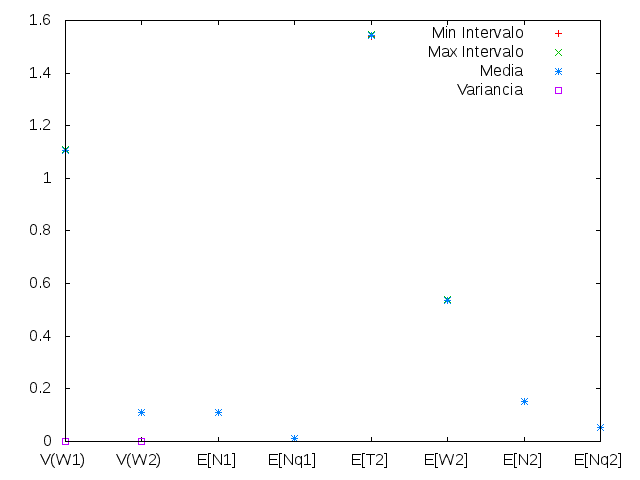
\includegraphics[width=1\textwidth]{graphs/graph-2.png}
%   }\caption{Exemplo de uma figura}
%\end{figure}



%%%%%%%%%%%%%
% Otimização
%%%%%%%%%%%%%
\chapter{Otimização}

\section{Apresentação do Método}

\section{Análise Gráfica de Resultados}

%%%%%%%%%%%%%
% Conclusão
%%%%%%%%%%%%%
\chapter{Conclusão}


%%%%%%%%%%%%%%%%%%%
% parte final
%%%%%%%%%%%%%%%%%%%

\appendix
\chapter{O Programa}

\section{Workflow}

\textbf{Modelo}

\tikzstyle{decision} = [diamond, draw, fill=blue!20, text width=4.5em, text badly centered, node distance=4cm, inner sep=0pt]
\tikzstyle{block} = [rectangle, draw, fill=blue!20, text width=5em, text centered, rounded corners, minimum height=4em]
\tikzstyle{line} = [draw, -latex']
\tikzstyle{cloud} = [draw, ellipse,fill=red!20, node distance=5cm, minimum height=2em]
    
\begin{tikzpicture}[node distance = 3cm, auto]
    % Place nodes
    \node [block] (init) {initialize model};
    \node [cloud, left of=init] (expert) {expert};
    \node [cloud, right of=init] (system) {system};
    \node [block, below of=init] (identify) {identify candidate models};
    \node [block, below of=identify] (evaluate) {evaluate candidate models};
    \node [block, left of=evaluate, node distance=3cm] (update) {update model};
    \node [decision, below of=evaluate] (decide) {is best candidate better?};
    \node [block, below of=decide, node distance=3cm] (stop) {stop};
    % Draw edges
    \path [line] (init) -- (identify);
    \path [line] (identify) -- (evaluate);
    \path [line] (evaluate) -- (decide);
    \path [line] (decide) -| node [near start] {yes} (update);
    \path [line] (update) |- (identify);
    \path [line] (decide) -- node {no}(stop);
    \path [line,dashed] (expert) -- (init);
    \path [line,dashed] (system) -- (init);
    \path [line,dashed] (system) |- (evaluate);
\end{tikzpicture}

\section{Diagrama de Classes}

\textbf{Modelo}

\tikzstyle{abstract}=[rectangle, draw=black, rounded corners, fill=blue!40, drop shadow,
        text centered, anchor=north, text=white, text width=3cm]
\tikzstyle{comment}=[rectangle, draw=black, rounded corners, fill=green, drop shadow,
        text centered, anchor=north, text=white, text width=3cm]
\tikzstyle{myarrow}=[->, >=open triangle 90, thick]
\tikzstyle{line}=[-, thick]

\begin{center}
\begin{tikzpicture}[node distance=2cm]
    \node (Item) [abstract, rectangle split, rectangle split parts=2]
        {
            \textbf{ITEM}
            \nodepart{second}name
        };
    \node (AuxNode01) [text width=4cm, below=of Item] {};
    \node (Component) [abstract, rectangle split, rectangle split parts=2, left=of AuxNode01]
        {
            \textbf{COMPONENT}
            \nodepart{second}nil
        };
    \node (System) [abstract, rectangle split, rectangle split parts=2, right=of AuxNode01]
        {
            \textbf{SYSTEM}
            \nodepart{second}parts
        };
    \node (AuxNode02) [text width=0.5cm, below=of Component] {};
    \node (Sensor) [abstract, rectangle split, rectangle split parts=2, left=of AuxNode02]
        {
            \textbf{SENSOR}
            \nodepart{second}nil
        };
    \node (Part) [abstract, rectangle split, rectangle split parts=2, right=of AuxNode02]
        {
            \textbf{PART}
            \nodepart{second}nil
        };
        
    \node (AuxNode03) [below=of Sensor] {};
    \node (Pressure) [abstract, rectangle split, rectangle split parts=2, left=of AuxNode03, xshift=2cm]
        {
            \textbf{Pressure}
            \nodepart{second}nil
        };
    \node (Temperature) [abstract, rectangle split, rectangle split parts=2, right=of AuxNode03, xshift=-2cm]
        {
            \textbf{Temperature}
            \nodepart{second}nil
        };
    \node (PressureInstants) [comment, rectangle split, rectangle split parts=2, below=0.2cm of Pressure, text justified]
        {
            \textbf{Instants}
            \nodepart{second}fw-p-suction\newline fw-p-delivery\newline fw-p-loop\newline sw-p-suction\newline sw-p-delivery
                \newline sw-p-loop
        };
    \node (ClOp) [abstract, rectangle split, rectangle split parts=2, below=0.4cm of PressureInstants]
        {
            \textbf{Closed/Open}
            \nodepart{second}nil
        };
    \node (ClOpInstants) [comment, rectangle split, rectangle split parts=2, below=0.2cm of ClOp, text justified]
        {
            \textbf{Instants}
            \nodepart{second}fw-clop-warm-up\newline sw-clop-control
        };
    \node (TemperatureInstants) [comment, rectangle split, rectangle split parts=2, below=0.2cm of Temperature, text justified]
        {
            \textbf{Instants}
            \nodepart{second}fw-t-engine\newline fw-t-heat-exch.\newline sw-t-heat-exch.
        };
    \node (Level) [abstract, rectangle split, rectangle split parts=2, below=0.4cm of TemperatureInstants]
        {
            \textbf{Level}
            \nodepart{second}nil
        };
    \node (LevelInstants) [comment, rectangle split, rectangle split parts=2, below=0.2cm of Level, text justified]
        {
            \textbf{Instants}
            \nodepart{second}fw-l-tank
        };
    \node (Ammeter) [abstract, rectangle split, rectangle split parts=2, below=0.4cm of LevelInstants]
        {
            \textbf{Ammeter}
            \nodepart{second}nil
        };
    \node (AmmeterInstants) [comment, rectangle split, rectangle split parts=2, below=0.2cm of Ammeter, text justified]
        {
            \textbf{Instants}
            \nodepart{second}fw-pump-ammeter\newline sw-pump-ammeter
        };
        
    \node (AuxNode04) [below=of Part] {};
    \node (Pump) [abstract, rectangle split, rectangle split parts=2, left=of AuxNode04, xshift=2cm]
        {
            \textbf{Pump}
            \nodepart{second}nil
        };
    \node (Valve) [abstract, rectangle split, rectangle split parts=2, right=of AuxNode04, xshift=-2cm]
        {
            \textbf{Valve}
            \nodepart{second}nil
        };
    \node (PumpInstants) [comment, rectangle split, rectangle split parts=2, below=0.2cm of Pump, text justified]
        {
            \textbf{Instants}
            \nodepart{second}fw-pump\newline sw-pump
        };
    \node (Tank) [abstract, rectangle split, rectangle split parts=2, below=0.4cm of PumpInstants]
        {
            \textbf{Tank}
            \nodepart{second}nil
        };
    \node (ValveInstants) [comment, rectangle split, rectangle split parts=2, below=0.2cm of Valve, text justified]
        {
            \textbf{Instants}
            \nodepart{second}fw-suction-valve\newline fw-delivery-valve\newline sw-suction-valve\newline sw-delivery-valve
                \newline sw-discharge-valve\newline sw-control-valve
        };
    \node (Engine) [abstract, rectangle split, rectangle split parts=2, below=0.4cm of ValveInstants]
        {
            \textbf{Engine}
            \nodepart{second}nil
        };
    \node (TankInstants) [comment, rectangle split, rectangle split parts=2, below=0.2cm of Tank, text justified]
        {
            \textbf{Instants}
            \nodepart{second}fw-expansion-tank
        };
    \node (HeatExchanger) [abstract, rectangle split, rectangle split parts=2, below=0.4cm of TankInstants]
        {
            \textbf{Heat Exchanger}
            \nodepart{second}nil
        };
    \node (HeatExchangerInstants) [comment, rectangle split, rectangle split parts=2, below=0.2cm of HeatExchanger, text justified]
        {
            \textbf{Instants}
            \nodepart{second}fw-heat-exchanger
        };
    \node (EngineInstants) [comment, rectangle split, rectangle split parts=2, below=0.2cm of Engine, text justified]
        {
            \textbf{Instants}
            \nodepart{second}fw-engine
        };
    \node (Strainer) [abstract, rectangle split, rectangle split parts=2, below=0.4cm of HeatExchangerInstants]
        {
            \textbf{Strainer}
            \nodepart{second}nil
        };
    \node (StrainerInstants) [comment, rectangle split, rectangle split parts=2, below=0.2cm of Strainer, text justified]
        {
            \textbf{Instants}
            \nodepart{second}sw-strainer
        };
    \node (Coolant) [abstract, rectangle split, rectangle split parts=2, below=0.4cm of EngineInstants]
        {
            \textbf{Coolant}
            \nodepart{second}nil
        };
    \node (CoolantInstants) [comment, rectangle split, rectangle split parts=2, below=0.2cm of Coolant, text justified]
        {
            \textbf{Instants}
            \nodepart{second}fw-coolant\newline sw-coolant
        };  

    \node (AuxNode05) [below=of System] {};
    \node (CoolingSystem) [abstract, rectangle split, rectangle split parts=2, left=of AuxNode05, xshift=2cm]
        {
            \textbf{Cooling System}
            \nodepart{second}nil
        };
    \node (CoolingLoop) [abstract, rectangle split, rectangle split parts=2, right=of AuxNode05, xshift=-2cm]
        {
            \textbf{Cooling Loop}
            \nodepart{second}nil
        };
    \node (CoolingSystemInstants) [comment, rectangle split, rectangle split parts=2, below=0.2cm of CoolingSystem, text justified]
        {
            \textbf{Instants}
            \nodepart{second}cool
        };
    \node (CoolingLoopInstants) [comment, rectangle split, rectangle split parts=2, below=0.2cm of CoolingLoop, text justified]
        {
            \textbf{Instants}
            \nodepart{second}fw-loop\newline sw-loop
        };
    
    \draw[myarrow] (Component.north) -- ++(0,0.8) -| (Item.south);
    \draw[line] (Component.north) -- ++(0,0.8) -| (System.north);
    
    \draw[myarrow] (Sensor.north) -- ++(0,0.8) -| (Component.south);
    \draw[line] (Sensor.north) -- ++(0,0.8) -| (Part.north);
    
    \draw[line] (Pressure.west) -- ++(-0.2,0);
    \draw[line] (Temperature.east) -- ++(0.2,0);
    \draw[line] (Level.east) -- ++(0.2,0);
    \draw[myarrow] (ClOp.west) -- ++(-0.2,0) -- ([yshift=0.5cm, xshift=-0.2cm] Pressure.north west) -|
     ([xshift=-1cm]Sensor.south);
    \draw[myarrow] (Ammeter.east) -- ++(0.2,0) -- ([yshift=0.5cm, xshift=0.2cm] Temperature.north east) -|
     ([xshift=1cm]Sensor.south);
     
    \draw[line] (Tank.west) -- ++(-0.2,0);
    \draw[line] (HeatExchanger.west) -- ++(-0.2,0);
    \draw[line] (Pump.west) -- ++(-0.2,0);
    \draw[line] (Valve.east) -- ++(0.2,0);
    \draw[line] (Engine.east) -- ++(0.2,0);
    \draw[myarrow] (Strainer.west) -- ++(-0.2,0) -- ([yshift=0.5cm, xshift=-0.2cm] Pump.north west) -|
     ([xshift=-1cm]Part.south);
    \draw[myarrow] (Coolant.east) -- ++(0.2,0) -- ([yshift=0.5cm, xshift=0.2cm] Valve.north east) -|
     ([xshift=1cm]Part.south);
     
    \draw[myarrow] (CoolingSystem.north) -- ++(0,0.8) -| (System.south);
    \draw[line] (CoolingSystem.north) -- ++(0,0.8) -| (CoolingLoop.north);
        
        
\end{tikzpicture}
\end{center}

\end{document}          
